% define \title (only used by writelatex.com)
%\title{CSEC-793 Project Report_Blank}
%%%%%%%%%%%%%%%%%%%%%%%%%%%%%%%%%%%%%%%%%%%%%%%%%%%%%%%%%%%%%%%%%%%%%%
% LaTeX Template: Project Titlepage
%
% Source: http://www.howtotex.com
% Date: April 2011
% 
% This is a title page template which be used for articles & reports.
% 
% Feel free to distribute this example, but please keep the referral
% to howtotex.com
% 
%%%%%%%%%%%%%%%%%%%%%%%%%%%%%%%%%%%%%%%%%%%%%%%%%%%%%%%%%%%%%%%%%%%%%%
% How to use writeLaTeX: 
%
% You edit the source code here on the left, and the preview on the
% right shows you the result within a few seconds.
%
% Bookmark this page and share the URL with your co-authors. They can
% edit at the same time!
%
% You can upload figures, bibliographies, custom classes and
% styles using the files menu.
%
% If you're new to LaTeX, the wikibook is a great place to start:
% http://en.wikibooks.org/wiki/LaTeX
%
%%%%%%%%%%%%%%%%%%%%%%%%%%%%%%%%%%%%%%%%%%%%%%%%%%%%%%%%%%%%%%%%%%%%%%
%
% --------------------------------------------------------------------
% Preamble
% --------------------------------------------------------------------
\documentclass[ fontsize=11pt,twoside]{scrartcl}	% KOMA

\usepackage[letterpaper,pdftex]{geometry}	% A4paper margins
\setlength{\oddsidemargin}{5mm}			% Remove 'twosided' indentation
\setlength{\evensidemargin}{5mm}

\usepackage[english]{babel}
\usepackage[protrusion=true,expansion=true]{microtype}	
\usepackage{amsmath,amsfonts,amsthm,amssymb}
\usepackage{graphicx}
\usepackage{pseudocode}

\usepackage[latin1]{inputenc}
\usepackage{tikz}
\usetikzlibrary{shapes,arrows}


% --------------------------------------------------------------------
% Definitions (do not change this)
% --------------------------------------------------------------------
\newcommand{\HRule}[1]{\rule{\linewidth}{#1}} 	% Horizontal rule

\makeatletter							% Title
\def\printtitle{%						
    {\centering \@title\par}}
\makeatother									

\makeatletter							% Author
\def\printauthor{%					
    {\centering \Large \@author}}				
\makeatother							

% --------------------------------------------------------------------
% Metadata (Change this)
% --------------------------------------------------------------------
\title{	\Large \textsc{ CS-GY 9053 Intro to Java \\ 
															Project Report} 	% Subtitle
		 	\\[2.0cm]								% 2cm spacing
			\HRule{2pt} \\						% Upper rule
			\LARGE \textbf{\uppercase{Finance Manager Desktop App}}	% Title
			\HRule{2pt} \\ [0.5cm]		% Lower rule + 0.5cm spacing
			\Large \today			% Todays date
		}

 \author{
		Flavjo  Xhelollari\\	
		NYU Tandon School of Engineering\\
        Spring 2023
        \texttt{fx2078@nyu.edu} \\
}


\begin{document}
% ------------------------------------------------------------------------------
% Maketitle
% ------------------------------------------------------------------------------
\thispagestyle{empty}		% Remove page numbering on this page

\printtitle					% Print the title data as defined above
  	\vfill
\printauthor				% Print the author data as defined above
\newpage
% ------------------------------------------------------------------------------
% Begin document
% ------------------------------------------------------------------------------
\setcounter{page}{1}		% Set page numbering to begin on this page


%%%%%%%%%%%%%%%
%														%
% 			Main Contents            %
%														%
%%%%%%%%%%%%%%%

\section{About}

This project is a Java-based desktop application for managing finances through a user-friendly graphical interface. It utilizes a database to store and retrieve financial data, allowing users to track expenses, income, and overall financial health. The app also includes features such as budget planning and analysis, and it is designed to be customizable and scalable for a variety of personal finance needs.
\section{Code Structure}

The project consists of the following classes:

\begin{itemize}
\item Budget.java
\item BudgetDialog.java
\item BudgetManager.java
\item Export.java 
\item FinanceManagerGUI.java
\item Login.java
\item Search.java
\item Transaction.java
\item TransactionManager.java

\end{itemize}

\section{Screenshots}

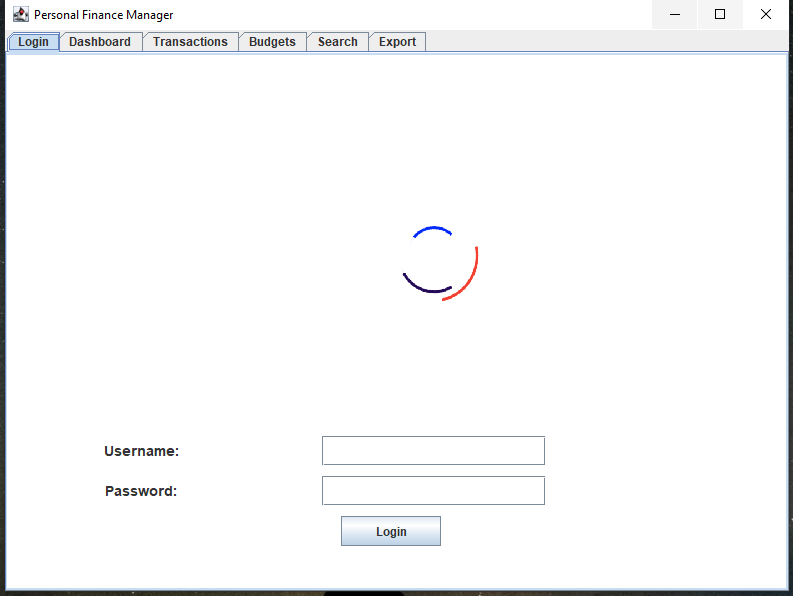
\includegraphics[width=0.89\textwidth]{login.png} \\

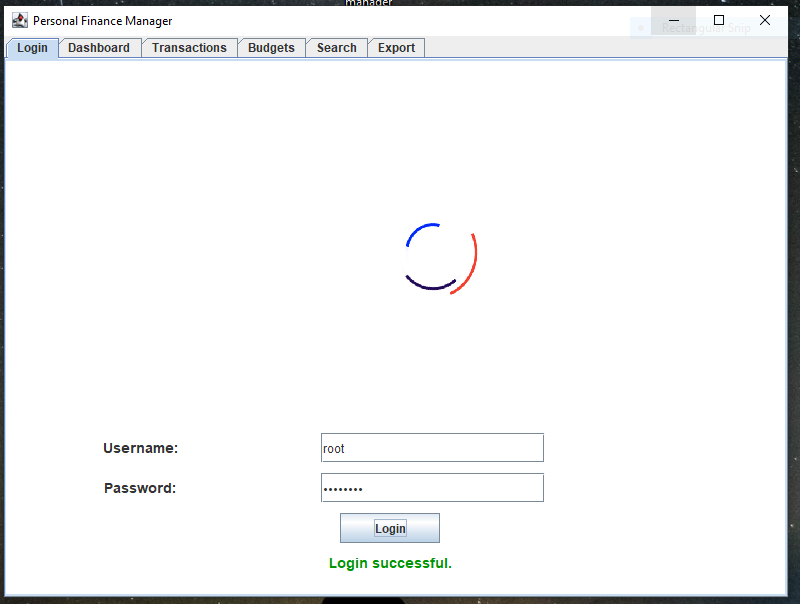
\includegraphics[width=0.89\textwidth]{login_successful.png} \\

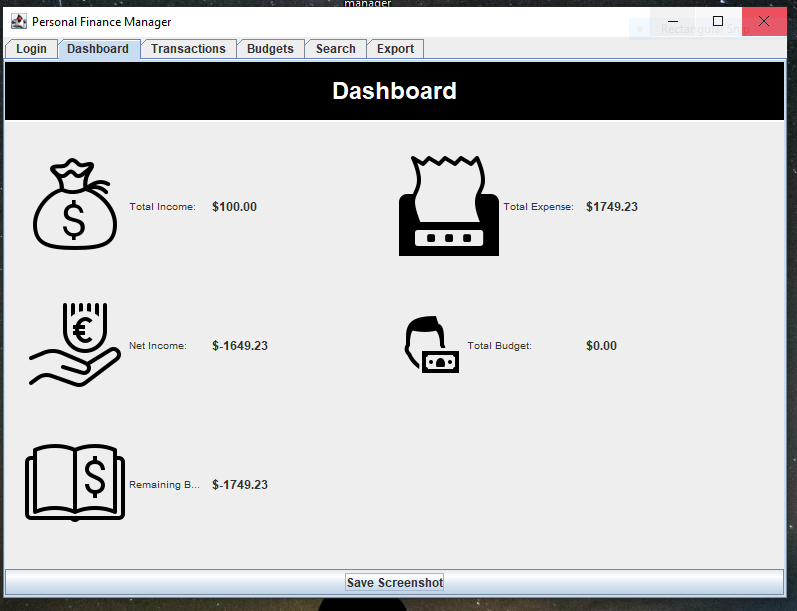
\includegraphics[width=0.89\textwidth]{dashboard.png} \\ 

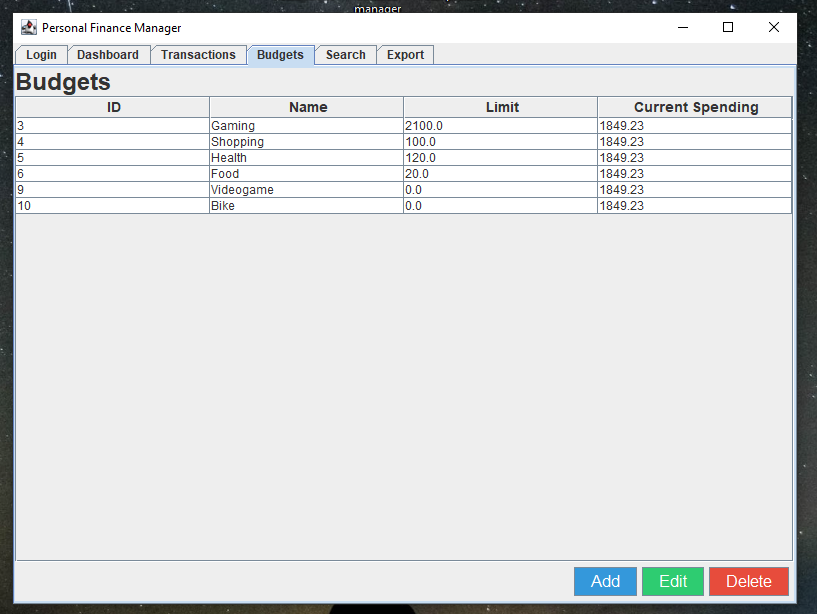
\includegraphics[width=0.89\textwidth]{budgets.png} \\ 

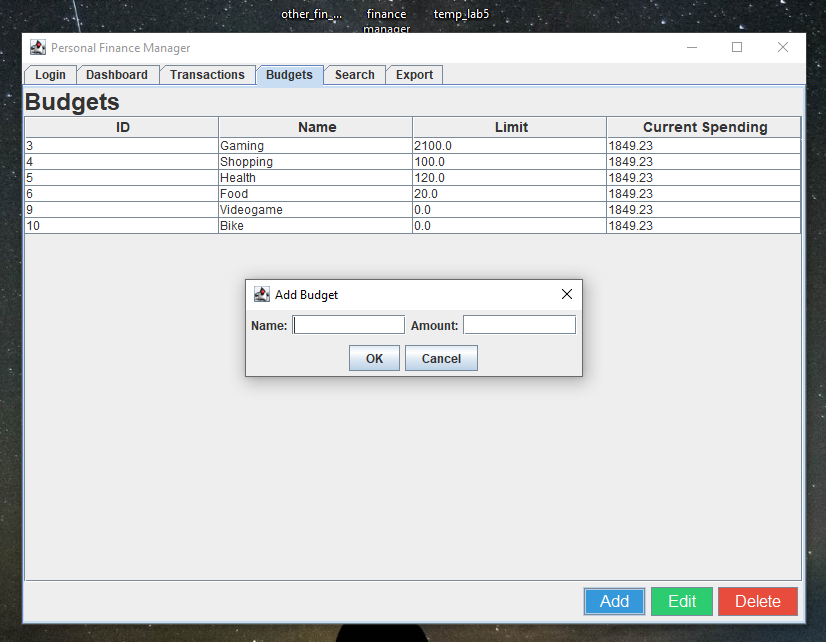
\includegraphics[width=0.89\textwidth]{budget_add.png} \\ 

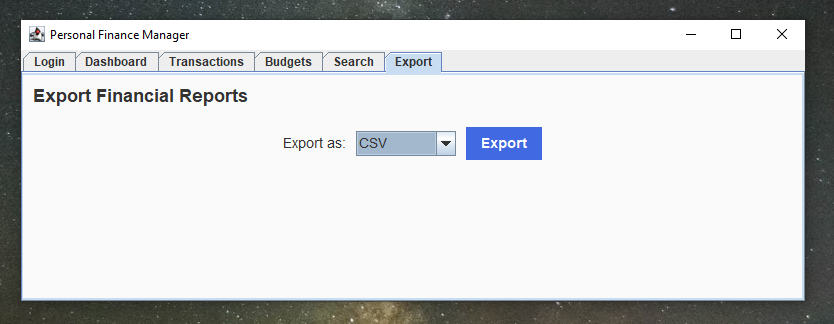
\includegraphics[width=0.89\textwidth]{export.png} \\ 

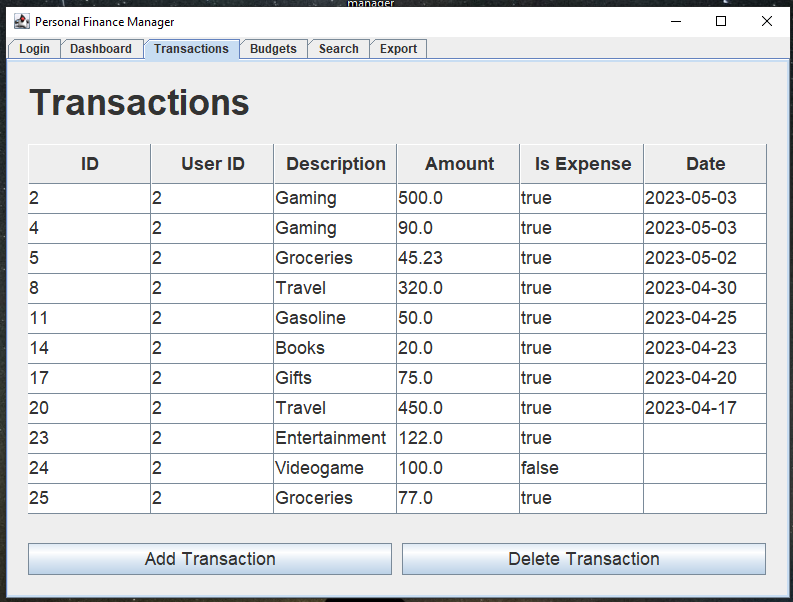
\includegraphics[width=0.89\textwidth]{transactions.png} \\

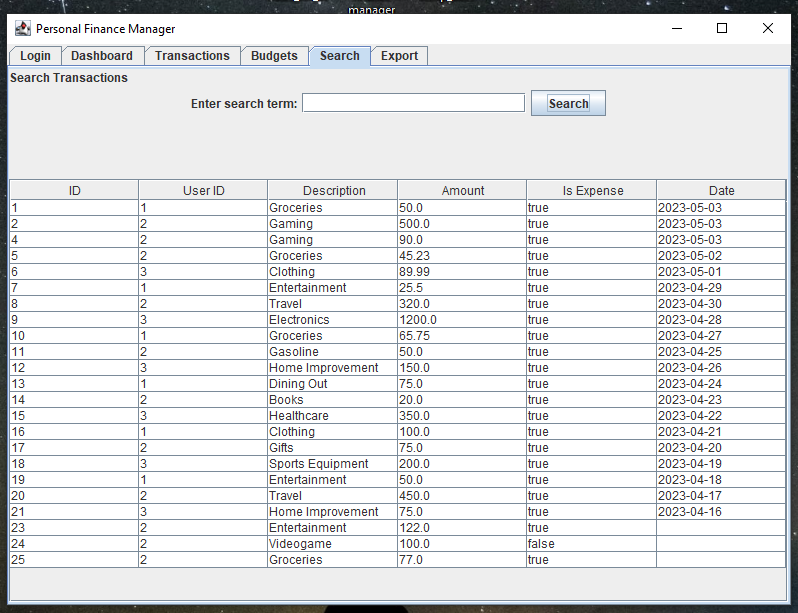
\includegraphics[width=0.89\textwidth]{transactions_search.png}
\section{Project description}

% In this section, first  redefine the problem in great details. Then describe your solutions. Try to use as many illustrations such as pictures, graphs, pseudo code as you see fit. Here are some examples of including pictures, graphs, and pseudo code in LaTeX. 

% %%%%%%%%%%%%%%%%%%%%%%%%%%%%%%%%%%%%%%%%%%%%%%%%%%%%%%%%%%%%%%%%%%%
% %
% % Commands to include a figure:
% %
% %%%%%%%%%%%%%%%%%%%%%%%%%%%%%%%%%%%%%%%%%%%%%%%%%%%%%%%%%%%%%%%%%%%
% Figure~\ref{fig:fig1} shows how to include a picture in a LaTeX document. 
% \begin{figure}[!ht]
%  \centering
% 
\includegraphics[width=3in]{sample_1}
% \caption{\label{fig:fig1}This is my great security design.}
% \end{figure}

% %%%%%%%%%%%%%%%%%%%%%%%%%%%%%%%%%%%%%%%%%%%%%%%%%%%%%%%%%%%%%%%%%%%
% %
% % The following pseudo code is copied from 
% % http://users.sdsc.edu/~ssmallen/latex/pseudocode.html
% %
% %%%%%%%%%%%%%%%%%%%%%%%%%%%%%%%%%%%%%%%%%%%%%%%%%%%%%%%%%%%%%%%%%%%
% Figure~\ref{fig:fig2} is a sample pseudo code copied from this site \cite{pseudocode}. 

% \begin{figure}[!ht]
%  \centering

%   \begin{pseudocode}[framebox]{reduce}{projection, x, y, f}
%     \FOR i \GETS 1 \TO y/f \DO
%       \BEGIN
%       \FOR j \GETS 1 \TO x/f \DO
%         \BEGIN
%         sum \GETS 0 \\
%         \FOR m \GETS 1 \TO f \DO
%           \BEGIN
%           \FOR n \GETS 1 \TO f \DO
%             sum = sum + projection[i*f+m][j * f+n]  \\
%           \END \\
%         reducedProjection[i][j] = sum / (f * f) \\
%         \END
%       \END \\
%   \RETURN{reducedProjection}
%   \end{pseudocode}
  
%   \caption{\label{fig:fig2}This is my great pseudo code}
  
%   \end{figure}
  
% %%%%%%%%%%%%%%%%%%%%%%%%%%%%%%%%%%%%%%%%%%%%%%%%%%%%%%%%%%%%%%%%%%%
% %
% % Latex float chart example
% % Copied from http://www.texample.net/tikz/examples/simple-flow-chart/
% %
% %%%%%%%%%%%%%%%%%%%%%%%%%%%%%%%%%%%%%%%%%%%%%%%%%%%%%%%%%%%%%%%%%%%

% Figure~\ref{fig:fig3} is a sample float chart is copied from this website \cite{floatchart}

% \tikzstyle{decision} = [diamond, draw, fill=blue!20, 
%     text width=4.5em, text badly centered, node distance=3cm, inner sep=0pt]
% \tikzstyle{block} = [rectangle, draw, fill=blue!20, 
%     text width=5em, text centered, rounded corners, minimum height=4em]
% \tikzstyle{line} = [draw, -latex']
% \tikzstyle{cloud} = [draw, ellipse,fill=red!20, node distance=3cm,
%     minimum height=2em]
   
%   \begin{figure}[!ht]
%  \centering
 
% \begin{tikzpicture}[node distance = 2cm, auto]
%     % Place nodes
%     \node [block] (init) {initialize model};
%     \node [cloud, left of=init] (expert) {expert};
%     \node [cloud, right of=init] (system) {system};
%     \node [block, below of=init] (identify) {identify candidate models};
%     \node [block, below of=identify] (evaluate) {evaluate candidate models};
%     \node [block, left of=evaluate, node distance=3cm] (update) {update model};
%     \node [decision, below of=evaluate] (decide) {is best candidate better?};
%     \node [block, below of=decide, node distance=3cm] (stop) {stop};
%     % Draw edges
%     \path [line] (init) -- (identify);
%     \path [line] (identify) -- (evaluate);
%     \path [line] (evaluate) -- (decide);
%     \path [line] (decide) -| node [near start] {yes} (update);
%     \path [line] (update) |- (identify);
%     \path [line] (decide) -- node {no}(stop);
%     \path [line,dashed] (expert) -- (init);
%     \path [line,dashed] (system) -- (init);
%     \path [line,dashed] (system) |- (evaluate);
% \end{tikzpicture}

%   \caption{\label{fig:fig3}This is my great float chart}
  
%   \end{figure}


% %%%%%%%%%%%%%%%%%%%%%%%%%%%%%%%%%%%%%%%%%%%%%%%%%%%%%%%%%%%%%%%%%%%

% \subsection{Mathematics}

% If your project idea needs mathematics to formulate your methods, \LaTeX{} is great at typesetting mathematics. Let $X_1, X_2, \ldots, X_n$ be a sequence of independent and identically distributed random variables with $\text{E}[X_i] = \mu$ and $\text{Var}[X_i] = \sigma^2 < \infty$, and let
% $$S_n = \frac{X_1 + X_2 + \cdots + X_n}{n}
%       = \frac{1}{n}\sum_{i}^{n} X_i$$
% denote their mean. Then as $n$ approaches infinity, the random variables $\sqrt{n}(S_n - \mu)$ converge in distribution to a normal $\mathcal{N}(0, \sigma^2)$.

\section{Project implementation}
In this s
\section{Conclusion}
In this section,


% ------------------------------------------------------------------------------
% End document
% ------------------------------------------------------------------------------
\end{document}